\documentclass[12pt,a4paper]{article}

% ─── Page Layout ───────────────────────────────────────────────────────────────
\usepackage[a4paper, margin=0.8in, headheight=14pt]{geometry}

% ─── Fonts (XeLaTeX) ───────────────────────────────────────────────────────────
\usepackage{fontspec}
\usepackage{unicode-math}
\setmainfont{TeX Gyre Pagella}
\setmonofont[Scale=0.88]{TeX Gyre Cursor}
\setmathfont{Latin Modern Math}

% ─── Packages ──────────────────────────────────────────────────────────────────
\usepackage{xcolor}
\usepackage{colortbl}
\usepackage{titlesec}
\usepackage{enumitem}
\usepackage{tabularx}
\usepackage{longtable}
\usepackage{booktabs}
\usepackage{array}
\usepackage{amsmath}
\usepackage{tikz}
\usetikzlibrary{shapes.geometric, arrows.meta, positioning, calc, fit, decorations.pathreplacing, patterns}
\usepackage{tcolorbox}
\tcbuselibrary{skins, breakable}
\usepackage{hyperref}
\usepackage{fancyhdr}
\usepackage{graphicx}
\usepackage{microtype}
\hyphenpenalty=10000
\exhyphenpenalty=10000
\sloppy
\usepackage{caption}
\usepackage{setspace}
\usepackage{multirow}
\usepackage{tocloft}

% ─── Q&A helper ────────────────────────────────────────────────────────────────
\newcommand{\Q}[1]{\textbf{#1}\par\noindent\ignorespaces}

% ─── Colour Palette ────────────────────────────────────────────────────────────
\definecolor{myred}{RGB}{196,30,58}
\definecolor{mydark}{RGB}{30,30,50}
\definecolor{mygreen}{RGB}{14,120,80}
\definecolor{myteal}{RGB}{0,130,140}
\definecolor{myamber}{RGB}{180,100,0}
\definecolor{mypurple}{RGB}{100,30,160}
\definecolor{mygray}{RGB}{246,247,249}
\definecolor{mgframe}{RGB}{180,185,200}
\definecolor{watermark}{RGB}{145,150,170}
\definecolor{hdrred}{RGB}{250,232,235}
\definecolor{hdrgreen}{RGB}{220,244,233}
\definecolor{hdrteal}{RGB}{220,242,244}
\definecolor{hdramber}{RGB}{253,242,215}
\definecolor{hdrpurple}{RGB}{238,228,255}
\definecolor{hdrgray}{RGB}{238,240,245}

% ─── Section Formatting ────────────────────────────────────────────────────────
\titleformat{\section}
  {\large\bfseries\color{myred}}{\thesection.}{0.5em}{}
  [\vspace{1pt}{\color{myred}\rule{\linewidth}{0.8pt}}]
\titleformat{\subsection}
  {\normalsize\bfseries\color{myteal}}{\thesubsection}{0.5em}{}
\titlespacing*{\section}{0pt}{18pt}{7pt}
\titlespacing*{\subsection}{0pt}{11pt}{4pt}

% ─── Paragraph ─────────────────────────────────────────────────────────────────
\setlength{\parindent}{0pt}
\setlength{\parskip}{4pt}

% ─── TOC Styling ───────────────────────────────────────────────────────────────
\renewcommand{\cfttoctitlefont}{\large\bfseries\color{myred}}
\renewcommand{\cftaftertoctitle}{\par\noindent{\color{myred}\rule{\linewidth}{0.8pt}}}
\setlength{\cftbeforetoctitleskip}{0pt}
\setlength{\cftaftertoctitleskip}{6pt}
\renewcommand{\cftsecfont}{\normalsize\bfseries\color{mydark}}
\renewcommand{\cftsecpagefont}{\normalsize\bfseries\color{mydark}}
\renewcommand{\cftsecleader}{\cftdotfill{\cftdotsep}}
\setlength{\cftbeforesecskip}{7pt}
\renewcommand{\cftsubsecfont}{\small\color{mydark}}
\renewcommand{\cftsubsecpagefont}{\small\color{mydark}}
\setlength{\cftbeforesubsecskip}{3pt}
\setlength{\cftsubsecindent}{1.4em}

% ─── Table helpers ─────────────────────────────────────────────────────────────
\renewcommand{\arraystretch}{1.45}
\setlength{\tabcolsep}{6pt}
\arrayrulecolor{mydark}
\newcolumntype{B}[1]{>{\small\bfseries\raggedright\arraybackslash}m{#1}}
\newcolumntype{Y}{>{\small\raggedright\arraybackslash}X}
\renewcommand{\tabularxcolumn}[1]{m{#1}}

% ─── Header / Footer ───────────────────────────────────────────────────────────
\pagestyle{fancy}
\fancyhf{}
\fancyhead[L]{\small\color{myred}\textbf{BS-B401}\;\color{mydark}--- Biology for Engineers}
\fancyhead[R]{\small\color{myteal}\textbf{Module 3 Notes}}
\fancyfoot[C]{\small\color{mydark}\thepage}
\fancyfoot[R]{\small\color{watermark}\textit{\copyright\ Biraj Sarkar (CGEC)}}
\renewcommand{\headrulewidth}{0.5pt}
\renewcommand{\footrulewidth}{0.3pt}

% ─── Hyperref ──────────────────────────────────────────────────────────────────
\hypersetup{
  colorlinks=true, linkcolor=myteal, urlcolor=myteal,
  pdfauthor={Biraj Sarkar (CGEC)},
  pdftitle={BS-B401 --- Module 3 Notes: Genetics}
}

% ─── tcolorbox styles ──────────────────────────────────────────────────────────
\tcbset{
  tikzbox/.style={
    colback=mygray, colframe=mgframe, boxrule=0.6pt, arc=4pt,
    left=8pt, right=8pt, top=6pt, bottom=6pt,
    colbacktitle=mgframe, coltitle=mydark, fonttitle=\small\bfseries
  },
  defbox/.style={
    colback=hdrgreen, colframe=mygreen, boxrule=0.8pt, arc=4pt,
    left=9pt, right=9pt, top=6pt, bottom=6pt,
    colbacktitle=mygreen, coltitle=white, fonttitle=\small\bfseries
  },
  formulabox/.style={
    colback=hdrteal, colframe=myteal, boxrule=0.8pt, arc=4pt,
    left=9pt, right=9pt, top=7pt, bottom=7pt,
    colbacktitle=myteal, coltitle=white, fonttitle=\small\bfseries
  },
  examplebox/.style={
    colback=hdramber, colframe=myamber, boxrule=0.8pt, arc=4pt,
    left=9pt, right=9pt, top=6pt, bottom=6pt,
    colbacktitle=myamber, coltitle=white, fonttitle=\small\bfseries
  },
  masonbox/.style={
    colback=hdrpurple, colframe=mypurple, boxrule=0.8pt, arc=4pt,
    left=9pt, right=9pt, top=6pt, bottom=6pt,
    colbacktitle=mypurple, coltitle=white, fonttitle=\small\bfseries
  },
  exambox/.style={
    colback=hdrpurple, colframe=mypurple, boxrule=1pt, arc=5pt,
    left=10pt, right=10pt, top=8pt, bottom=8pt,
    colbacktitle=mypurple, coltitle=white, fonttitle=\bfseries,
    breakable, title after break={\textbf{Frequently Asked / Viva Questions (contd.)}}
  }
}
\tcbset{breakable}
\tcbset{after={\par\color{black}}}

% ─── TikZ styles ───────────────────────────────────────────────────────────────
\tikzset{
  block/.style={rectangle, draw=myteal, fill=hdrteal,
    text width=2.4cm, align=center, minimum height=0.95cm,
    font=\small, rounded corners=3pt, line width=0.7pt},
  redblock/.style={rectangle, draw=myred, fill=hdrred,
    text width=2.4cm, align=center, minimum height=0.95cm,
    font=\small, rounded corners=3pt, line width=0.7pt},
  amberblock/.style={rectangle, draw=myamber, fill=hdramber,
    text width=2.4cm, align=center, minimum height=0.95cm,
    font=\small, rounded corners=3pt, line width=0.7pt},
  sumjunc/.style={circle, draw=myamber, fill=hdramber,
    minimum size=0.62cm, font=\small, line width=0.8pt},
  arrow/.style={-Stealth, thick, color=mydark},
  redarrow/.style={-Stealth, thick, color=myred},
  line/.style={thick, color=mydark}
}

\begin{document}

% ─── Title Page ───────────────────────────────────────────────────────────────
\begin{center}
  {\LARGE\bfseries\color{myred} BS-B401 --- Biology for Engineers}\\[5pt]
  {\normalsize\color{mydark} Semester IV \quad$\bullet$\quad 2L:1T:0P \quad$\bullet$\quad 3 Credits}\\[3pt]
  {\normalsize\color{myteal}\textbf{Module 3 Exam Notes: Genetics}}\\[3pt]
  {\small\color{mydark} CGEC \;$|$\; B.Tech ECE (2023--27) \;$|$\; \textit{Biraj Sarkar}}
\end{center}
\vspace{2pt}
\noindent{\color{myred}\rule{\linewidth}{1.5pt}}
\vspace{2pt}

\hypersetup{linkcolor=mydark}
\tableofcontents
\hypersetup{linkcolor=myteal}
\newpage

\section{Genetics}
\subsection{Gene, allele and trait}
\begin{tcolorbox}[defbox, title={Foundations of heredity}]
A gene is a unit of heredity associated with a functional product. An allele is a variant of a gene at a particular locus, or chromosome position. Genotype is the genetic constitution being described. Phenotype is the observable trait and can depend on genotype, environment and development.
\end{tcolorbox}

\begin{itemize}[leftmargin=*, itemsep=3pt, topsep=4pt]
  \item \textbf{Diploid inheritance.} Two homologous chromosomes usually carry the same loci, one inherited from each parent. A homozygote has the same allele at a locus. A heterozygote has different alleles there.
  \item \textbf{Dominance.} With complete dominance, the heterozygote has the same scored phenotype as one homozygote. The other allele is recessive for that phenotype. Dominance says nothing about population frequency or fitness.
  \item \textbf{Other relationships.} In incomplete dominance the heterozygote is intermediate. In codominance both allele products are distinguishable, as with the A and B antigens of the human ABO blood group.
\end{itemize}
\subsection{Mendel's laws and predictions}
\begin{enumerate}[leftmargin=*, itemsep=3pt, topsep=4pt]
  \item \textbf{Segregation.} The two alleles at a locus separate during gamete formation. For a simple $Aa$ parent, each type of gamete normally carries one allele, with probabilities $1/2$ each.
  \item \textbf{Independent assortment.} Allele pairs at different unlinked loci assort independently. An $AaBb$ parent makes $AB$, $Ab$, $aB$ and $ab$ gametes in equal proportions under this condition.
  \item \textbf{Fertilisation.} One gamete from each parent combines to restore the diploid number. Multiply independent probabilities and add probabilities of mutually exclusive paths to the same outcome.
\end{enumerate}
\begin{tcolorbox}[examplebox, title={Monohybrid and dihybrid crosses}]
\par\vspace{5pt}
\begingroup
\setlength{\extrarowheight}{1pt}
\noindent\begin{tabularx}{\linewidth}{|B{3.5cm}|Y|Y|}
\hline
\textbf{Cross} & \textbf{Genotypes or gametes} & \textbf{Phenotypes under complete dominance} \\ \hline
$Aa\times Aa$ & $AA:Aa:aa=1:2:1$. The two routes to $Aa$ each contribute $1/4$. & Dominant to recessive $=3:1$. \\ \hline
$AaBb\times AaBb$ & Each parent makes four equally likely gametes if the loci are unlinked. & $A\_B\_:A\_bb:aaB\_:aabb=9:3:3:1$. \\ \hline
$Aa\times aa$ & Progeny $Aa:aa=1:1$. & A testcross uses the recessive homozygote to reveal the alleles in the other parent's gametes. \\ \hline
\end{tabularx}\par
\endgroup
For the dihybrid cross, $P(A\_B\_)=(3/4)(3/4)=9/16$ and $P(aabb)=(1/4)(1/4)=1/16$. Here an underscore means either allele in that position. The prediction assumes independent assortment, complete dominance and no viability differences.
\end{tcolorbox}

\subsection{What mitosis and meiosis transmit}
\begin{tcolorbox}[tikzbox, title={Genetic transmission across generations}]
\centering
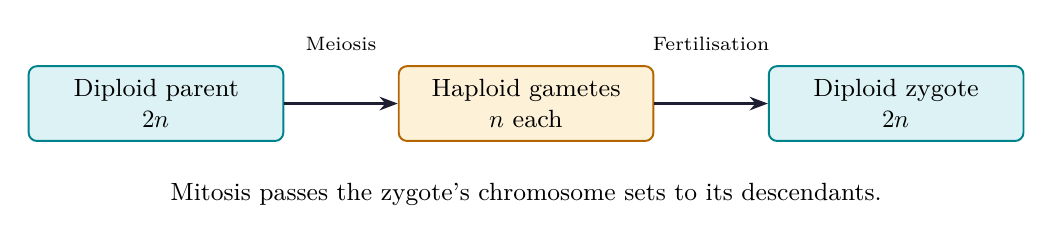
\begin{tikzpicture}[every node/.style={font=\small}]
\node[block,text width=3cm] (p) at (0,0) {Diploid parent\\$2n$};
\node[amberblock,text width=3cm] (g) at (4.7,0) {Haploid gametes\\$n$ each};
\node[block,text width=3cm] (z) at (9.4,0) {Diploid zygote\\$2n$};
\draw[arrow] (p)--(g);
\draw[arrow] (g)--(z);
\node[font=\scriptsize] at (2.35,0.76) {Meiosis};
\node[font=\scriptsize] at (7.05,0.76) {Fertilisation};
\node at (4.7,-1.15) {Mitosis passes the zygote's chromosome sets to its descendants.};
\end{tikzpicture}\par
\end{tcolorbox}

\par\vspace{5pt}
\begingroup
\setlength{\extrarowheight}{1pt}
\noindent\begin{tabularx}{\linewidth}{|B{3cm}|Y|Y|}
\hline
\textbf{Feature} & \textbf{Mitosis} & \textbf{Meiosis} \\ \hline
Primary role & Growth, maintenance and asexual cell proliferation. & Form haploid cells for sexual reproduction or for a haploid life stage. \\ \hline
Chromosome sets & Preserves ploidy in ordinary division. & One replication followed by two divisions reduces diploid to haploid. \\ \hline
What separates & Sister chromatids separate. & Homologues separate first. Sister chromatids then separate. \\ \hline
Diversity & Daughter cells are usually genetically similar. & Independent orientation and crossing over can produce new allele combinations. \\ \hline
\end{tabularx}\par
\endgroup
\section{Linkage, Gene Interaction and Human Inheritance}
\subsection{Linkage and gene mapping}
Linked loci on the same chromosome can be inherited together more often than predicted by independent assortment. Crossing over between homologous chromosomes creates recombinant combinations.
\begin{tcolorbox}[examplebox, title={Map two loci using a testcross}]
A heterozygote $AB/ab$ is crossed with $ab/ab$. The counts for $AB,ab,Ab,aB$ gametes are 420, 420, 80 and 80. The rare types are recombinant.
\[
\text{Recombination fraction}=\frac{80+80}{1000}=0.16.
\]
A short-interval estimate is about 16 map units (centimorgans). A two-point recombination fraction approaches at most 50\% even when multiple crossovers occur, so it may underestimate large map distances.
\end{tcolorbox}

\subsection{Gene interaction and epistasis}
\begin{tcolorbox}[defbox, title={Epistasis}]
Epistasis occurs when genotype at one locus changes or masks the phenotype expected at another locus. Dominance compares alleles at a single locus.
\end{tcolorbox}

\begin{tcolorbox}[examplebox, title={How recessive epistasis changes a ratio}]
Suppose $E$ permits pigment deposition and $ee$ prevents it. Among animals that can deposit pigment, $B\_$ gives dark colour and $bb$ gives brown colour. From a dihybrid cross, $9/16$ are $B\_E\_$, $3/16$ are $bbE\_$ and $4/16$ are $\_\_ee$. The phenotype ratio is $9:3:4$ because the two $ee$ classes look alike.
\end{tcolorbox}

\subsection{From phenotype to gene and complementation}
\begin{enumerate}[leftmargin=*, itemsep=3pt, topsep=4pt]
  \item \textbf{Record the phenotype.} Decide what is being scored and record variation and family relationships.
  \item \textbf{Infer a model.} Use segregation and pedigrees to predict dominant, recessive or other possible inheritance patterns.
  \item \textbf{Test the locus.} Ask whether the trait and nearby markers are inherited together. Recombination can narrow an interval. Independent functional evidence helps distinguish a causal gene from its neighbours.
\end{enumerate}
\par\vspace{5pt}
\begingroup
\setlength{\extrarowheight}{1pt}
\noindent\begin{tabularx}{\linewidth}{|B{3.2cm}|Y|Y|}
\hline
\textbf{Single-gene example} & \textbf{Inheritance typically taught} & \textbf{Biological link} \\ \hline
Cystic fibrosis & Autosomal recessive. & Pathogenic variants in \textit{CFTR} affect ion transport. \\ \hline
Sickle cell disease & Autosomal recessive inheritance for the HbSS example. & Variants of \textit{HBB} change beta-globin. Other allele combinations can also cause disease. \\ \hline
Huntington disease & Autosomal dominant. & An expanded repeat in \textit{HTT} contributes to progressive neurological disease. \\ \hline
\end{tabularx}\par
\endgroup
\begin{tcolorbox}[examplebox, title={Human genetics thought experiment: complementation}]
Two unrelated parents have similar recessive hearing phenotypes. Assume one is $aaBB$ and the other $AAbb$, and that a functional copy of both genes is needed for typical hearing. A child $AaBb$ has a functional copy at each locus and is predicted to complement. If the parents instead both have the same recessive cause, represented here as $aa$, their children would lack a functional $A$ allele. This simplified model explains why apparently similar phenotypes can involve different genes.
\end{tcolorbox}

\begin{tcolorbox}[masonbox, title={Use the assumptions}]
Complementation is interpreted for recessive variants under an appropriate loss-of-function model. Real pedigrees may also reflect penetrance, environment or more than one contributing locus.
\end{tcolorbox}

\textbf{Primary reading.} \href{https://doi.org/10.1534/genetics.116.195198}{Mendel's 1866 paper in English translation}.

\subsection{Build a Mendelian answer from the gametes}
\begin{tcolorbox}[examplebox, title={Read a Punnett square and account for each outcome}]
For $Aa\times Aa$, each parent contributes $A$ or $a$ with probability $1/2$. Each square has probability $1/4$.
\par\vspace{6pt}
\noindent\begin{tabularx}{\linewidth}{|B{3.5cm}|Y|Y|}
\hline
\textbf{Gamete from the first parent} & \textbf{$A$ from the second} & \textbf{$a$ from the second} \\ \hline
$A$ & $AA$ & $Aa$ \\ \hline
$a$ & $Aa$ & $aa$ \\ \hline
\end{tabularx}\par\smallskip

So $P(AA)=1/4$, $P(Aa)=1/2$, and $P(aa)=1/4$. With complete dominance, $AA$ and $Aa$ join in one phenotype class, giving $3:1$ while the genotype ratio remains $1:2:1$. Random inheritance can produce different counts in a small family.
\end{tcolorbox}

\subsection{Reason from a pedigree}
\begin{enumerate}[leftmargin=*, itemsep=2pt]
  \item \textbf{Propose a model.} Two unaffected parents have an affected child. Under the simple autosomal recessive model with complete penetrance, both parents can be $Aa$ carriers and the affected child is $aa$.
  \item \textbf{Predict a new outcome.} The probability of an affected child in another pregnancy is $1/4$ under that model.
  \item \textbf{Use conditional probability when needed.} If a child is known to be unaffected, exclude the $aa$ square. Two of the three equally likely remaining squares are $Aa$, giving carrier probability $2/3$.
  \item \textbf{Check the assumptions.} One short pedigree may fit several models. Other relatives, marker inheritance or functional evidence help distinguish them.
\end{enumerate}

\subsection{Why linkage and epistasis change different results}
\begin{itemize}[leftmargin=*, itemsep=2pt]
  \item \textbf{Linkage changes gamete frequencies.} A testcross may reveal two abundant parental combinations. Count both recombinant classes before using the recombination fraction.
  \item \textbf{Epistasis changes the phenotype grouping.} For the pigment example, $B\_ee$ contributes $3/16$ and $bbee$ contributes $1/16$. Both lack pigment deposition, so the two form one $4/16$ class. The two loci can still assort independently.
  \item \textbf{Complementation helps distinguish loci.} Two recessive defects may look similar because the affected genes contribute to the same task. Under the stated assumptions the offspring restores that task by inheriting a functional copy at each locus.
\end{itemize}

\newpage
\begin{center}
  {\large\bfseries\color{myred} Quick Revision --- Module 3}\\[3pt]
  {\small\color{mydark} Genetics $|$ BS-B401}
\end{center}
\noindent{\color{myred}\rule{\linewidth}{1.2pt}}\par\vspace{4pt}

\begin{tcolorbox}[formulabox, title={Key Concepts at a Glance}]
\renewcommand{\arraystretch}{1.35}
\noindent\begin{tabularx}{\linewidth}{B{4.5cm}Y}
Monohybrid cross & $Aa\times Aa$: genotype $1:2:1$ and, with complete dominance, phenotype $3:1$. \\[3pt]
Independent events & Multiply probabilities for independent gamete outcomes. \\[3pt]
Map distance & Recombinants divided by total progeny, converted to percentage for a short interval. \\[3pt]
\end{tabularx}\par
\end{tcolorbox}

\begin{tcolorbox}[defbox, title={One-Line Definitions}]
\begin{itemize}[leftmargin=*, itemsep=3pt, topsep=4pt]
  \item \textbf{Allele.} A variant at a genetic locus.
  \item \textbf{Epistasis.} Interaction in which one locus alters the phenotypic effect of another.
  \item \textbf{Complementation.} Restoration of function by combining variants that leave functional copies at different loci.
\end{itemize}
\end{tcolorbox}

\begin{tcolorbox}[exambox, title={Frequently Asked / Viva Questions}]
\begin{enumerate}[topsep=0pt, label=\textbf{Q\arabic*.}, itemsep=5pt, leftmargin=*]
  \item \Q{What segregates during gamete formation?}
    The two alleles at a locus.
  \item \Q{When is independent assortment a good prediction?}
    For unlinked loci, or loci effectively unlinked in the observed cross.
  \item \Q{What is a testcross?}
    A cross to a recessive homozygote to reveal gamete types.
  \item \Q{Does dominance mean commonness?}
    Dominance describes the phenotype of a heterozygote.
  \item \Q{Which division reduces ploidy?}
    Meiosis.
  \item \Q{Why can linked loci produce recombinants?}
    Crossing over can exchange material between homologues.
  \item \Q{What is a centimorgan?}
    A genetic map unit, approximated by one percent recombination over a short interval.
  \item \Q{Why can epistasis produce 9:3:4?}
    Two genotype categories merge because one genotype masks the other locus.
  \item \Q{What does a pedigree show?}
    Trait transmission across relatives and generations.
  \item \Q{What does two-locus complementation indicate under the simple model?}
    Each parent carries a different recessive cause. A functional copy at each locus restores the trait.
\end{enumerate}
\end{tcolorbox}

\begin{tcolorbox}[tikzbox, title={Summary Comparison}]
\par\vspace{5pt}
\begingroup
\setlength{\extrarowheight}{1pt}
\noindent\begin{tabularx}{\linewidth}{|B{3.45cm}|Y|Y|}
\hline
\textbf{Concept} & \textbf{Scale} & \textbf{Typical clue} \\ \hline
Dominance & One locus & Phenotype of a heterozygote. \\ \hline
Epistasis & Two or more loci & One locus masks or modifies another. \\ \hline
Linkage & Chromosome region & Parental gamete classes occur in excess. \\ \hline
\end{tabularx}\par
\endgroup
\end{tcolorbox}

\end{document}
